\section{Results}
\label{sec:res}
Model training is performed for all 25 companies in the AEX index, with five randomly sampled time periods for each of the models. This ensures there is enough data to answer the research questions. Although all parameters are kept consistent between model training, some errors do inevitably creep into the results necessitating result selection. MAPE scores equal or above 1.0, i.e. a +100\% error rate, are discarded, as these are obvious errors where the models did not perform as expected. With identical model training cycles, random samples seeded with identical values and identical training data, identical results were expected, but the reality is that results have to be manually selected to ensure quality. To assure each model is represented equally, 50 results were sampled from each model and plot our results.

\subsection{RQ1: The influence of pandemic features on stock pricing}
To fully answer the extent of this research question, first the performance of our models must be assessed in comparison to the baseline. During EDA and the results collection a sample of these results was taken from the training cycles and pair-plotted for quick comparison \ref{fig:samplefits}.
During EDA this study experimented with different sized ratios of training and testing data and determined a ten to one ratio of training vs. testing data should be sufficient. The target prediction length was seven days of values for the daily interval and three weeks of values for weekly interval. From the pair-plot model fittings some prediction errors can clearly be seen, but these are expected given the variance in the training data. It can also clearly be seen that the baseline model (labeled as "dummy") functions as expected, ignoring all input features except the last known value of the response variable.

\subsubsection{Model performance}
Given access to all features while implementing automatic feature selection, model performance on the MAPE metric is compared for daily and weekly data (see Figure \ref{fig:modelcompare}).
Weekly data generally shows higher error scores, especially for the ARIMA model. An unusual result is that none of the models show any noteworthy performance differences when compared to the baseline model. The baseline should average out to a small error score, but the expectation was that with sufficient training data and feature selection, the other models should've outperformed the baseline. In our sample fits a possible cause can be seen, as some results show extreme errors in predictions.

\subsubsection{Time period}
As a difference between daily and weekly data was established for predictions, the results can also distinguish the used time period for training and testing.
As the pandemic started at the end of 2019, it can be seen that the error scores increase in 2020 and consequently decrease in 2021. This could support the hypothesis that the pandemic caused an upset in 2020 and was restoring in 2021. An indication that this is not just an artifact of the pandemic data, there is little difference to be seen in the baseline model between 2019 and 2021, even though the pandemic is still widespread in the latter year. The same behaviour can also be seen on a weekly basis, indicating that this also generalizes over longer prediction periods.

%\begin{figure}
%    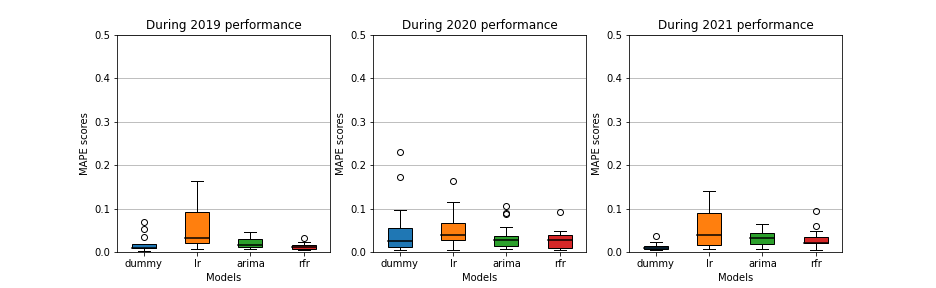
\includegraphics[width=.45\paperwidth]{thesis/images/plots/daily_2019_vs_2020_vs_2021_max_05.png}
%    \caption{Models trained on daily data, split by year, capped at MAPE score <= 0.5}
%    \label{fig:yearplot}
%\end{figure}

\begin{figure}
\centering
\begin{subfigure}[b]{.6\linewidth}
    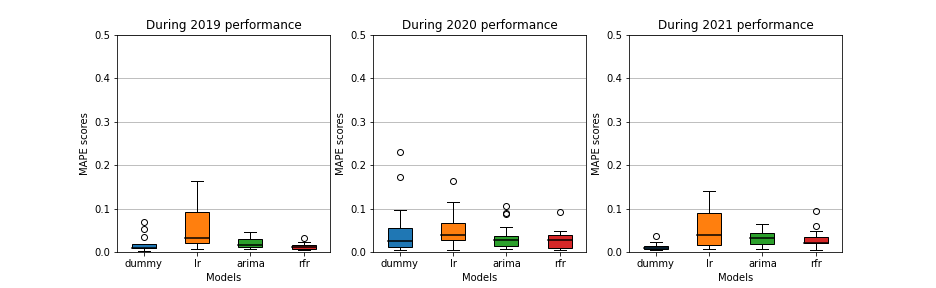
\includegraphics[width=\linewidth]{thesis/images/plots/daily_2019_vs_2020_vs_2021_max_05.png}
    \caption{Models trained on daily data, split by year, capped at MAPE score <= 0.5}
    \label{fig:yearplot}
\end{subfigure}
\begin{subfigure}[b]{.4\linewidth}
    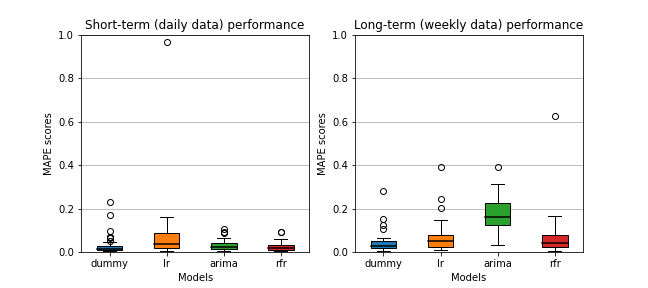
\includegraphics[width=\linewidth]{thesis/images/plots/base_model_comparison_daily_weekly.png}
    \caption{Daily data vs. weekly data}
    \label{fig:modelcompare}
\end{subfigure}
\begin{subfigure}[b]{.4\linewidth}
    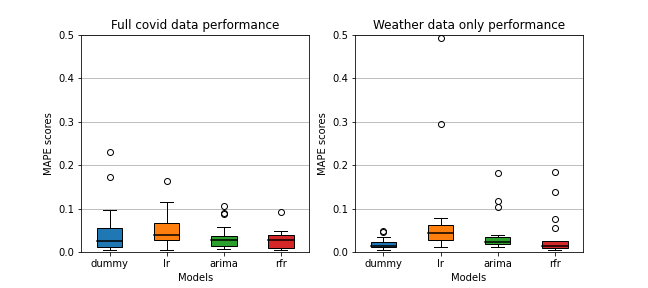
\includegraphics[width=\linewidth]{thesis/images/plots/daily_full_covid_data_vs_weather_data_only_max_05.png}
    \caption{The full dataset vs. weather data only}
    \label{fig:weathervfull}
\end{subfigure}

\begin{subfigure}[b]{.4\linewidth}
    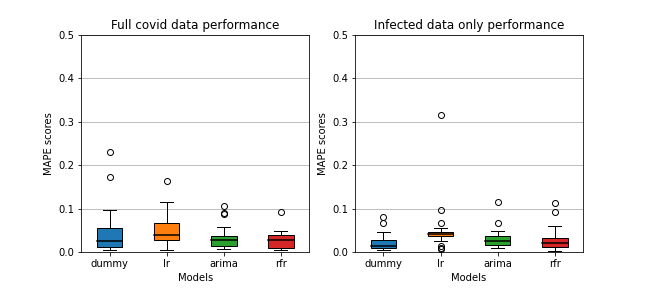
\includegraphics[width=\linewidth]{thesis/images/plots/daily_full_covid_data_vs_infected_data_only_max_05.png}
    \caption{The full dataset vs. COVID-19 infection data only}
    \label{fig:infectvfull}
\end{subfigure} 
\begin{subfigure}[b]{.4\linewidth}
    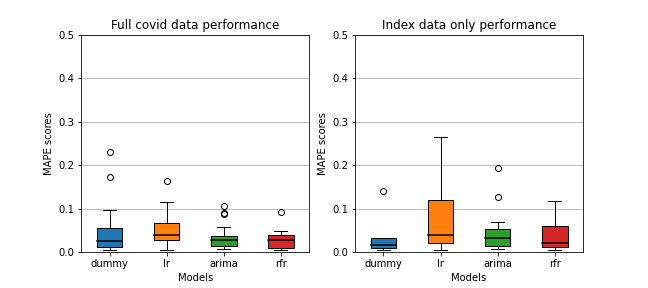
\includegraphics[width=\linewidth]{thesis/images/plots/daily_full_covid_data_vs_index_data_only_max_05.png}
    \caption{The full dataset vs. no additional features}
    \label{fig:indexvfull}
\end{subfigure}
\caption{Comparisons of model scores}
\end{figure}

\subsubsection{Feature performance}
To isolate the impact of data features on our error metric, the same predictions were ran given different selections of features. The results above were given full access to the data, but the following variables were isolated: Weather features, COVID-19- infections, -deaths, -partial/-full vaccinations, stringency of regulations \cite{hale2020variation} and no additional features.
Looking at a comparison of the MAPE scores between weather data only and the full dataset, there is no notable difference in performance (see Figure \ref{fig:weathervfull}). This could indicate that either the weather features are always selected during features selection, or none of the features are of any value to the models.
The latter could be true given none of the models show a notable performance increase from the baseline, but the feature of infections shows that pandemic data does have some influence (see Figure \ref{fig:infectvfull}), at least for the ARIMA and RFR models. The same can be said for deaths, vaccination data and the stringency index, where the ARIMA and RFR model (almost) outperform the baseline model. Although the differences are subtle, they are noticeable, especially compared to LR which shows consistent high error scores compared to the baseline. 
Weather features are the richest of all data and features can be seen as individual features. The only test left is one where the models are given no additional input features and only the response variable defines the output of the models. As a consequence all models increase in performance compared to the baseline as the number of data features decrease, posing the question whether any additional features is helpful at all (see Figure \ref{fig:indexvfull}). 

\begin{table}[h]
\hspace*{\fill}
\parbox{.45\columnwidth}{
\centering
\begin{tabular}{lllll|}
\cline{4-5}
\multicolumn{3}{l|}{}                                                                                                                        & \multicolumn{2}{l|}{\textbf{Baseline compare}} \\ \hline
\multicolumn{1}{|l|}{\textbf{Features}}                    & \multicolumn{1}{l|}{\textbf{Model}} & \multicolumn{1}{l|}{\textbf{MAPE}} & \multicolumn{1}{l|}{\textbf{t-stat}}  & \textbf{p} \\ \hline
\multicolumn{1}{|l|}{\multirow{2}{*}{\textbf{All}}} & \multicolumn{1}{|l|}{\textbf{ARIMA}}                      & 0.0302                                  & -0.3735                               & 0.7096     \\ \cline{2-5} 
\multicolumn{1}{|l|}{}                                       & \multicolumn{1}{|l|}{\textbf{RFR}}                        & 0.0234                                  & 0.6711                                & 0.5037     \\ \hline
\multicolumn{1}{|l|}{\multirow{2}{*}{\textbf{None}}}  & \multicolumn{1}{|l|}{\textbf{ARIMA}}                      & 0.0315                                  & -1.7365                               & 0.0856     \\ \cline{2-5} 
\multicolumn{1}{|l|}{}                                       & \multicolumn{1}{|l|}{\textbf{RFR}}                        & 0.0242                                  & -0.5310                               & 0.5966     \\ \hline
\end{tabular}
\caption{Model MAPE score comparison to baseline, for all dataset features and no additional features}
\label{tbl:modelscores}
}
\hfill
% \end{table}
\parbox{.45\columnwidth}{
\centering
% \begin{table}
\begin{tabular}{l|llll|}
\cline{2-5}
                                        & \multicolumn{1}{l|}{\textbf{Features: All}} & \multicolumn{1}{l|}{\textbf{None}} & \multicolumn{2}{l|}{\textbf{Comparison}}          \\ \hline
\multicolumn{1}{|l|}{\textbf{Model}}    & \multicolumn{1}{l|}{\textbf{MAPE}}    & \multicolumn{1}{l|}{\textbf{MAPE}}   & \multicolumn{1}{l|}{\textbf{t-stat}} & \textbf{p} \\ \hline
\multicolumn{1}{|l|}{\textbf{ARIMA}}    & 0.0341                                     & 0.0434                                    & -0.8300                              & 0.4114     \\ \hline
\multicolumn{1}{|l|}{\textbf{RFR}}      & 0.0300                                     & 0.0408                                    & -0.7865                              & 0.4380     \\ \hline
\multicolumn{1}{|l|}{\textbf{Baseline}} & 0.0475                                     & 0.253                                     & 1.3612                               & 0.1824     \\ \hline
\end{tabular}
\caption{Data feature MAPE score comparison for all the ARIMA, RFR and baseline models}
\label{tbl:datascores}
}
\hspace*{\fill}
\end{table}

\begin{figure}[H]
  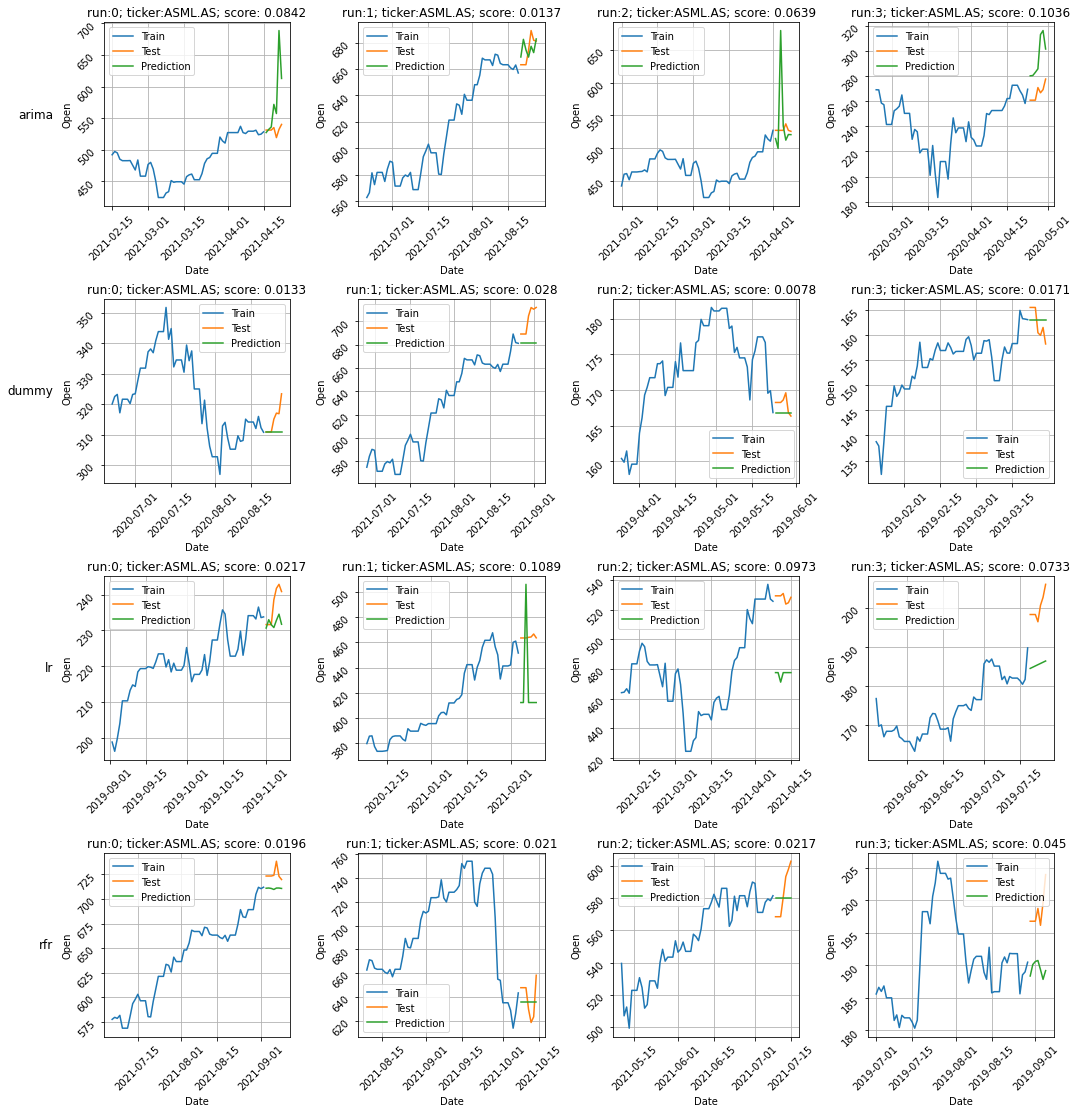
\includegraphics[width=0.9\textwidth]{images/plots/sample_fits_asml.png}
  \caption{Side-by-side model fittings and resulting daily predictions for ASML}
  \label{fig:samplefits}
\end{figure}

\subsection{RQ2: Performance of machine learning techniques in stock market prediction}
As the RFR model is considered as part of the machine learning techniques, it should be compared to the baseline and evaluated on its relative performance. The differences in performance are minute and necessitate an insight into the significance tests to give a reliable measure of difference in performance. For the sake of simplicity, this study has only done this comparison for the daily data, as the weekly data shows unreliable performance. Given a confidence level of 95\% ($\alpha = 0.05$), a T-test on the MAPE scores for the full dataset and the dataset containing no additional features results in the following table \ref{tbl:modelscores}.
With these results it can be said that there is no significant performance difference in using machine learning techniques such as RFR for stock market prediction. The same can be said for the ARIMA model, with the notion that ARIMA does seem to show better performance with reduced features. As each row in table \ref{tbl:modelscores} refers to an individual T-test, the dimensions can also be flipped to test whether the features in the data influence the models in table \ref{tbl:datascores}.
This research shows there is no significant difference in the mean MAPE error scores between all or no additional features in the data, for none of the models.